\documentclass[a4paper]{article}

\usepackage[utf8]{inputenc}
\usepackage[T1]{fontenc}
\usepackage{geometry}
\usepackage[francais]{babel}
\usepackage{graphicx}
\usepackage{fullpage}
\usepackage{hyperref}
\usepackage{amsfonts}
\usepackage{amsmath}
\usepackage[nottoc, notlof, notlot]{tocbibind}

%\pagestyle{headings}

\title{Projet Java}
\author{Simon Mauras}
\date{9 Janvier 2015}

\begin{document}
  
  \maketitle
  
  \tableofcontents

  \section{Introduction}
  
  Ce projet a été réalisé au cours du premier semestre de l'année de L3 au département d'informatique de l'ENS de Lyon. L'objectif étant de se familiariser avec le langage Java et différents algorithmes de Clustering.

Le sujet nous invitait dans un premier temps à réaliser une interface graphique de manière à valider le bon fonctionnement de notre implémentation en considérant un ensemble de points du plan. La seconde partie nous proposait un choix de différentes pistes à approfondir : utiliser un algorithme plus efficace pour le calcul des diagrammes de Voronoï, se placer dans un espace de dimension supérieure à 2 afin de pouvoir analyser des données de différents types, implémenter un algorithme de Clustering spectral, trouver une heuristique permettant de deviner le nombre optimal de Clusters, ...

J'ai choisi d'implémenter un algorithme suivant le paradigme "diviser pour régner" permettant de calculer une triangulation de Delaunay en temps $\mathcal O(n \log n)$. Avec cet algorithme, publié en 1980 par Lee et Schachter, il est possible de construire des diagrammes de Voronoï de manière efficace.

  \newpage
  
  \section{Organisation générale du projet}
  
  Dès le début du projet, j'ai essayé de bien séparer les classes responsables de l'interface graphique et les classes implémentant les différents algorithmes.

  \begin{figure}[h]
    \centering
    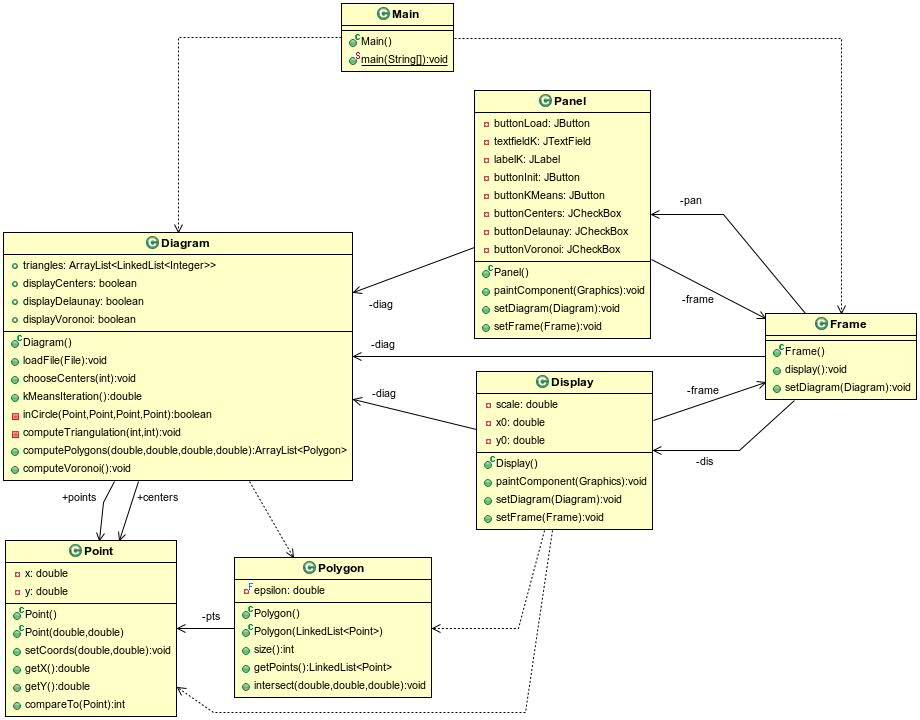
\includegraphics[width=15cm]{../UML.jpg}
    \caption{Diagramme UML du projet.}
  \end{figure}

  La classe \verb|Main| est appellée au début de l'exécution. Elle crée une instance de la classe \verb|Frame| (responsable de l'affichage graphique) et une instance de la classe \verb|Diagram| (effectuant les différents calculs).

  La classe \verb|Display| dessine les points et polygones, elle interagit avec la classe \verb|Diagram| (pour obtenir les donnée à afficher) et la classe \verb|Frame| (pour gérer le zoom et forcer le ré-affichage de la fenêtre).

  La classe \verb|Panel| contient les différents boutons et gère les évenements associés, elle interagit avec la classe \verb|Diagram| (pour lancer les différents calculs) et la classe \verb|Frame| (pour forcer le ré-affichage à la fin d'un calcul).

  La classe \verb|Diagram| implémente différents algorithmes (K-Moyennes, triangulation de Delaunay et diagramme de Voronoï). Elle est responsable de la lecture des données dans un fichier (\verb|loadFile|). Les structures \verb|Point| et \verb|Polygon| sont utilisées pour représenter les données. Les fonctions \verb|kMeansIteration| et \verb|computeDelaunay| sont appellées toutes les 100ms par la classe \verb|Panel| lorsqu'un calcul est en cours. La fonction \verb|computeVoronoi| est appellée par la classe \verb|Display| à chaque ré-affichage.

  \section{Lecture dans un fichier et algorithme des K-Moyennes}

  Nous avons choisi de pouvoir lire les points dans un fichier. Les générateurs (écrits en OCaml) ainsi que des données utilisées sont disponibles dans le dossier \verb|test|. Les différents générateurs couvrent des cas particuliers.

  \newpage

  \begin{figure}[!h]
    \centering
    \begin{tabular}{cc}
      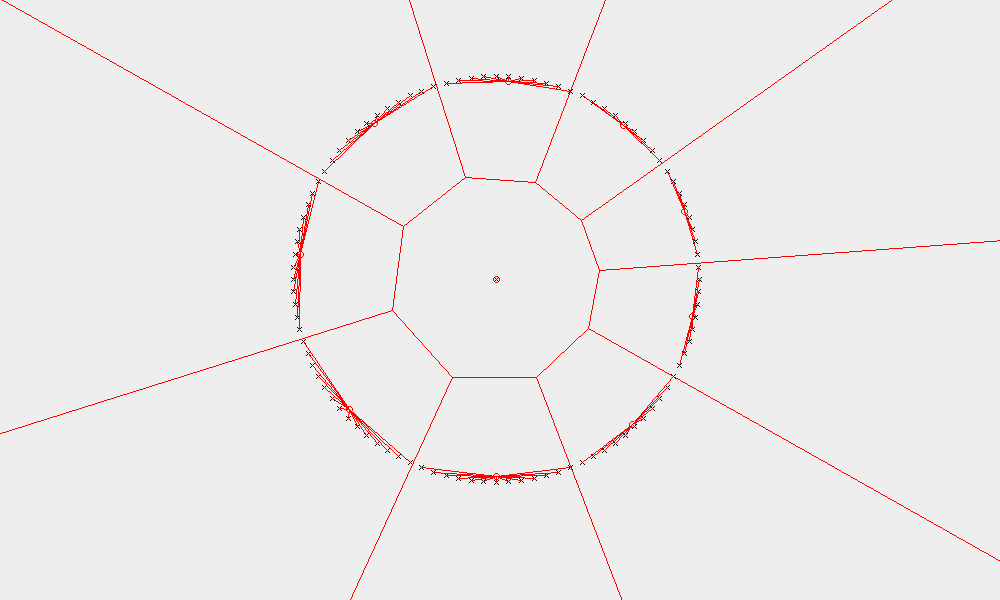
\includegraphics[width=8cm]{wheel.png} &
      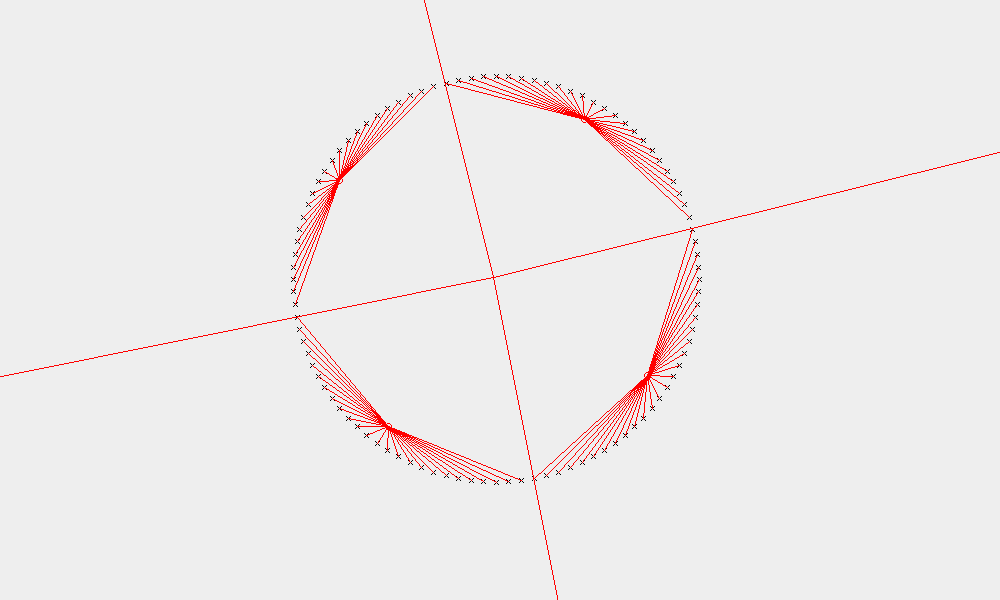
\includegraphics[width=8cm]{circle.png} \\
      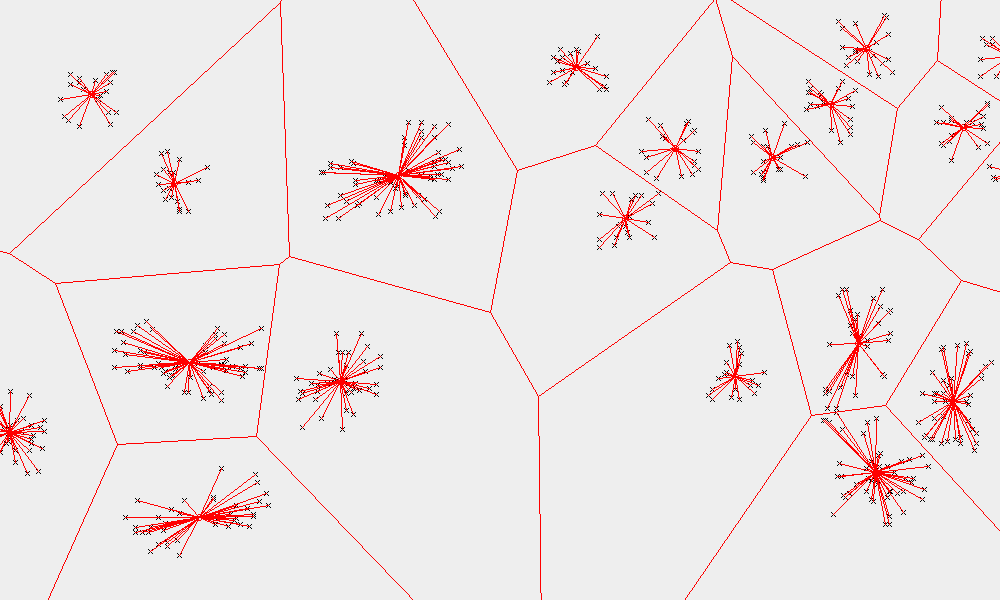
\includegraphics[width=8cm]{cluster.png} &
      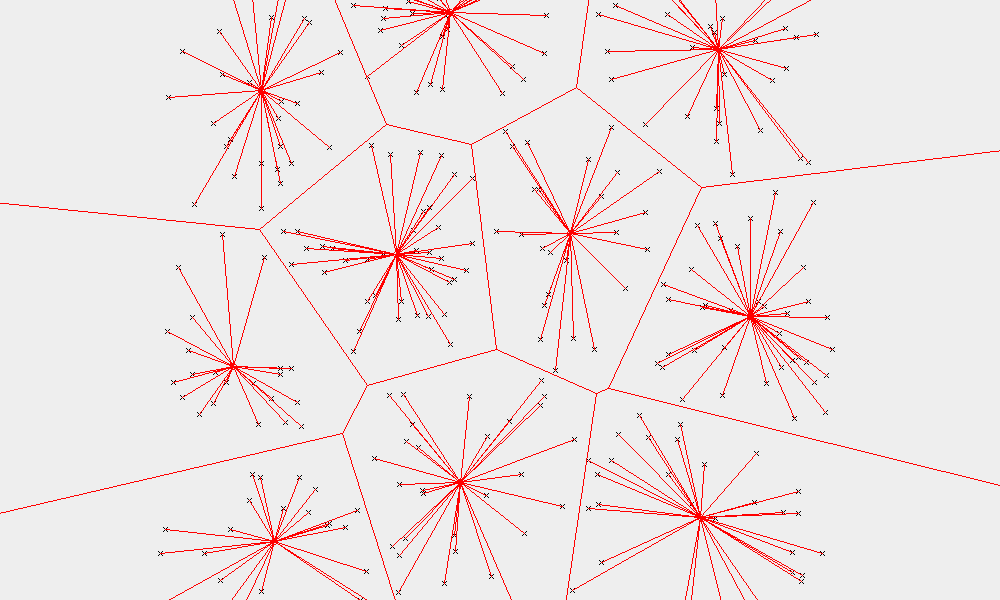
\includegraphics[width=8cm]{uniform.png} \\
    \end{tabular}
    \caption{Différents générateurs}
  \end{figure}

Les centres sont actuellement choisis de manière aléatoire parmis les points. La fonction \verb|kMeansIteration| effectue une seule modification des centres. L'animation consiste à itérer tant que la variation n'est pas devenue infime.

\section{Triangulation de Delaunay}

Une triangulation de Delaunay est le graphe dual d'un diagramme de Voronoï. Le passage de l'un à l'autre peut se faire de en temps linéaire. Nous avons décidé de commencer par calculer la triangulation de Delaunay de notre ensemble de centres avant de générer le diagramme de Voronoï, de manière à éviter les problèmes qui peuvent se poser avec les arrondis des nombres en virgule flottante.

L'algorithme que j'ai adopté est celui proposé par Lee et Schachter en 1980. Il s'agit d'un algorithme qui trie les sommets par abscisse croissante puis procède en suivant le paradigme "diviser pour régner" : il coupe l'ensemble en deux, calcule la triangulation dans les parties droite et gauche puis fusionne les deux en $\mathcal O(n)$. Une description plus complète est disponible en [1].

La principale difficulté que j'ai pu rencontrer est de bien comprendre comment gérer les cas ou plusieurs points ont la même abscisse, que ce soit pour le choix d'un ordre valide pour le tri et aussi lors de la fusion entre les parties gauche et droite qui s'effectue de bas en haut.

\section{Génération du diagramme de Voronoï}

Par la suite, générer le diagramme de Voronoï à partir d'une triangulation de Delaunay est en tout point identique à l'algorithme basique décrit dans le sujet à l'exception du fait qu'il nous suffit de calculer les intersection des demi-plans pour les voisins immédiats dans le graphe représentant la triangulation de Delaunay. Si on sait que le nombre d'arêtes dans un graphe planaire est linéaire en le nombre de sommet, le calcul de l'ensemble des cellules peut se faire de manière efficace.


  \begin{figure}[h]
    \centering
    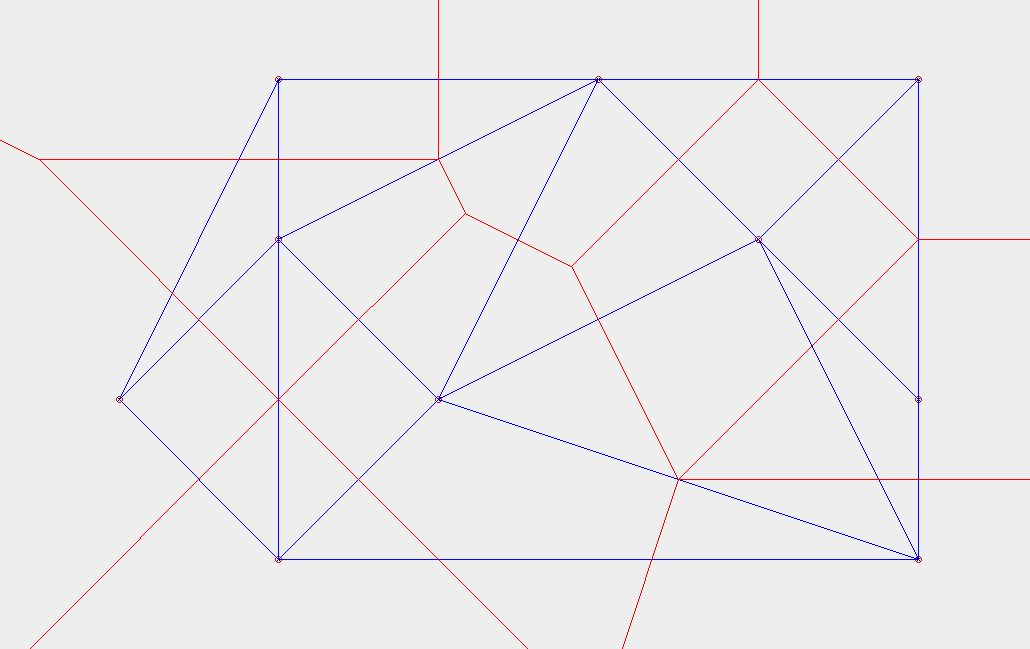
\includegraphics[width=15cm]{dual.png}
    \caption{La triangulation de Delaunay est le graphe dual du diagramme de Voronoi}
  \end{figure}

\section{Conclusion}

J'ai tiré de ce projet plusieurs points enrichissants. Parmis eux la satisfaction de s'être plongé dans un article de recherche pour comprendre en profondeur un algorithme assez complexe. J'ai également appris à organiser mon code de manière cohérente en séparant l'affichage des calculs (pattern MVC malgré une séparation peu marquée entre Vue et Contrôle).

\section{Références}

\begin{itemize}
\item D.T. Lee, B.J. Schachter, ``Two Algorithms for Constructing a Delaunay Triangulation'', \textit{International Journal of Computer and Information Sciences}, Jun 1980
\item S. Peterson, ``Computing constrained Delaunay triangulations'', \href{http://www.geom.uiuc.edu/~samuelp/del_project.html}{[en ligne, consulté en janvier 2015]}
\end{itemize}

\end{document}
